\section{Технологический раздел}

В данном разделе определяются инструменты разработки средства сбора данных и средства распознавания суицидальных паттернов поведения человека по текстовым сообщениям.
Представлены интерфейсы разработанных средств. Приведена информация о модулях системы.

Приводится описание обрабатываемых данных, а также анализ тональности сообщений и облаков слов каждого класса.

\subsection{Выбор инструментов разработки}

В качестве средства реализации средства сбора данных была выбрана библиотека Telebot, так как:

\begin{enumerate}
	\item[1.] Функционал приложения не предусматривает сложных операций, в силу чего низкая производительность ЯП Python не скажется на скорости отклика системы;
	\item[2.] ЯП Python позволит быстро разворачивать приложение на разнообразных операционных системах, поддерживающих интерпретатор Python;
	\item[3.] Telebot предоставляет более тонкую настройку и контроль над запросами и ответами API Telegram.
\end{enumerate}

Для организации хранения данных и моделей задействована реляционная СУБД PostgreSQL~\cite{postgres}. 
Данный выбор обусловлен наличием реляционных отношений в описанной системе, а также количеством полей у каждой сущности меньше 10, таким образом, данная СУБД может удовлетворить все потребности при реализации.

В качестве средства разработки метода распознавания суицидальных паттернов поведения человека по текстовым сообщениям использовался ЯП Python. Данный выбор обусловлен следующими факторами:

\begin{itemize}
	\item большое количество реализаций средств анализа и предобработки текста;
	\item широкий выбор библиотек для разработки в области машинного обучения;
	\item просто синтаксиса языка и высокая скорость разработки.
\end{itemize}

В качестве среды разработки был задействован Visual Studio Code. Данный выбор обусловлен тем, что это ПО распространяется по свободной лицензии, поставляется для конечного пользователя с открытым исходным кодом, а также имеет большое число расширений, ускоряющих процесс разработки.

Список задействованных в разработанном методе библиотек:
\begin{itemize}
	\item pandas~\cite{pandas} -- библиотека для обработки и анализа данных;
	\item numpy~\cite{numpy} -- библиотека, добавляющая поддержку больших многомерных массивов и матриц, вместе с большой библиотекой высокоуровневых математических функций для операций с этими массивами;
	\item matplotlib~\cite{matplotlib} -- библиотека для визуализации данных;
	\item scikit-learn~\cite{sklearn} -- библиотека множества операций и алгоритмов, используемых в сфере науки о данных и машинном обучении;
	\item nltk~\cite{nltk} -- библиотека, предоставляющая обширный набор инструментов для работы с естественными языками;
	\item pymorphy2~\cite{pymorphy} -- библиотека, предоставляющая морфологический анализатор, а также утилиты для взаимодействия с ним.
\end{itemize}

\subsection{Интерфейсы разработанных средств}

На рисунках \ref{img:teleg1}-\ref{img:teleg4} представлен интерфейс реализованного Telegram-бота.

\begin{figure}[H]
	\centering
	
\includegraphics[width=\textwidth]{inc/teleg1.png}
	\caption{ Приветственное сообщение новому пользователю. }
	\label{img:teleg1}
\end{figure}

\begin{figure}[H]
	\centering
	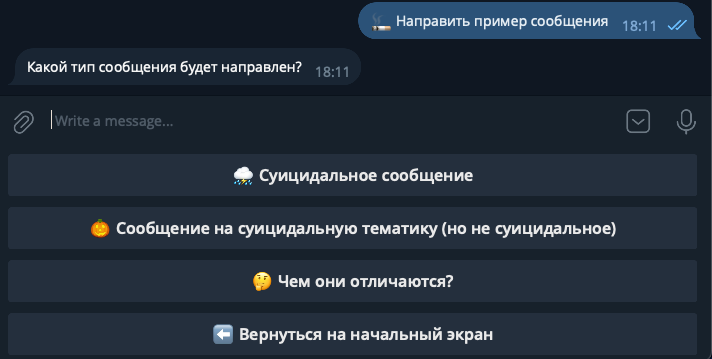
\includegraphics[width=\textwidth]{inc/teleg2.png}
	\caption{ Функционал направления в систему сообщения пользователем. }
	\label{img:teleg2}
\end{figure}

\begin{figure}[H]
	\centering
	
\includegraphics[width=\textwidth]{inc/teleg3.png}
	\caption{ Пример результата направленного в систему суицидального сообщения. }
	\label{img:teleg3}
\end{figure}

\begin{figure}[H]
	\centering
	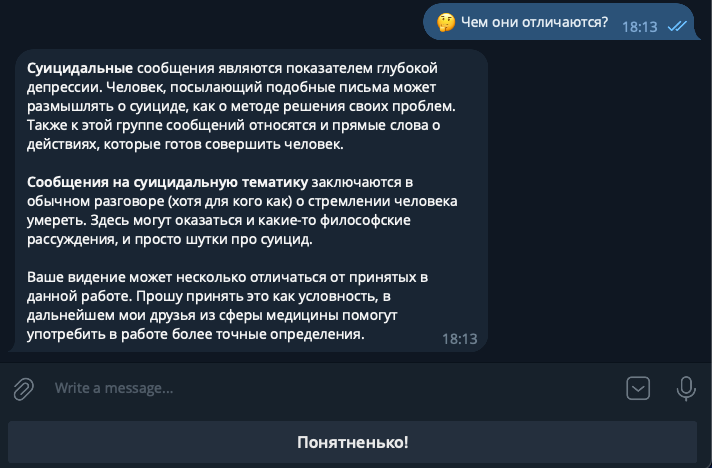
\includegraphics[width=\textwidth]{inc/teleg4.png}
	\caption{ Описание отличий суицидального сообщения и сообщения на суицидальную тематику. }
	\label{img:teleg4}
\end{figure}

На рисунках \ref{img:utility1}-\ref{img:utility4} представлен интерфейс реализованного средства распознавания суицидальных паттернов поведения человека по текстовым сообщениям. 
Средство позволяет выбрать пользователю как модель, так и метод векторизации сообщения, поступающего в систему.
Кроме того, предусмотрена возможность демонстрационного запуска, который позволяет получит результат работы всех доступных в средстве моделей.

\begin{figure}[H]
	\centering
	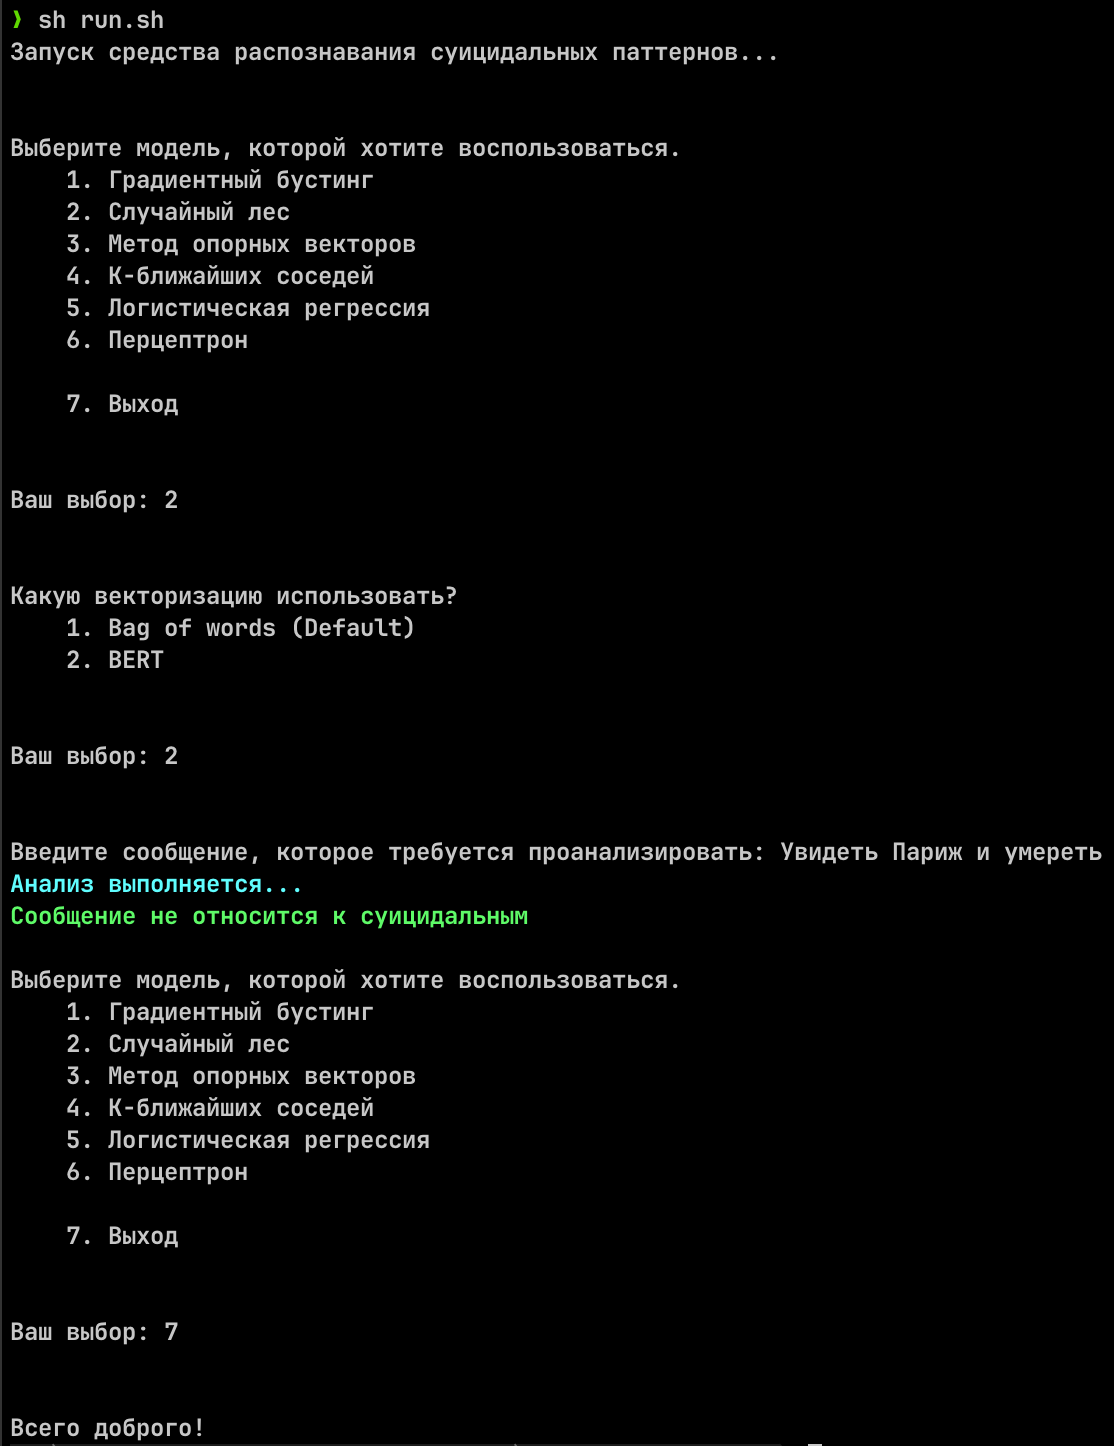
\includegraphics[width=\textwidth]{inc/utility1.png}
	\caption{ Полная пользовательская история использования средства. }
	\label{img:utility1}
\end{figure}

\begin{figure}[H]
	\centering
	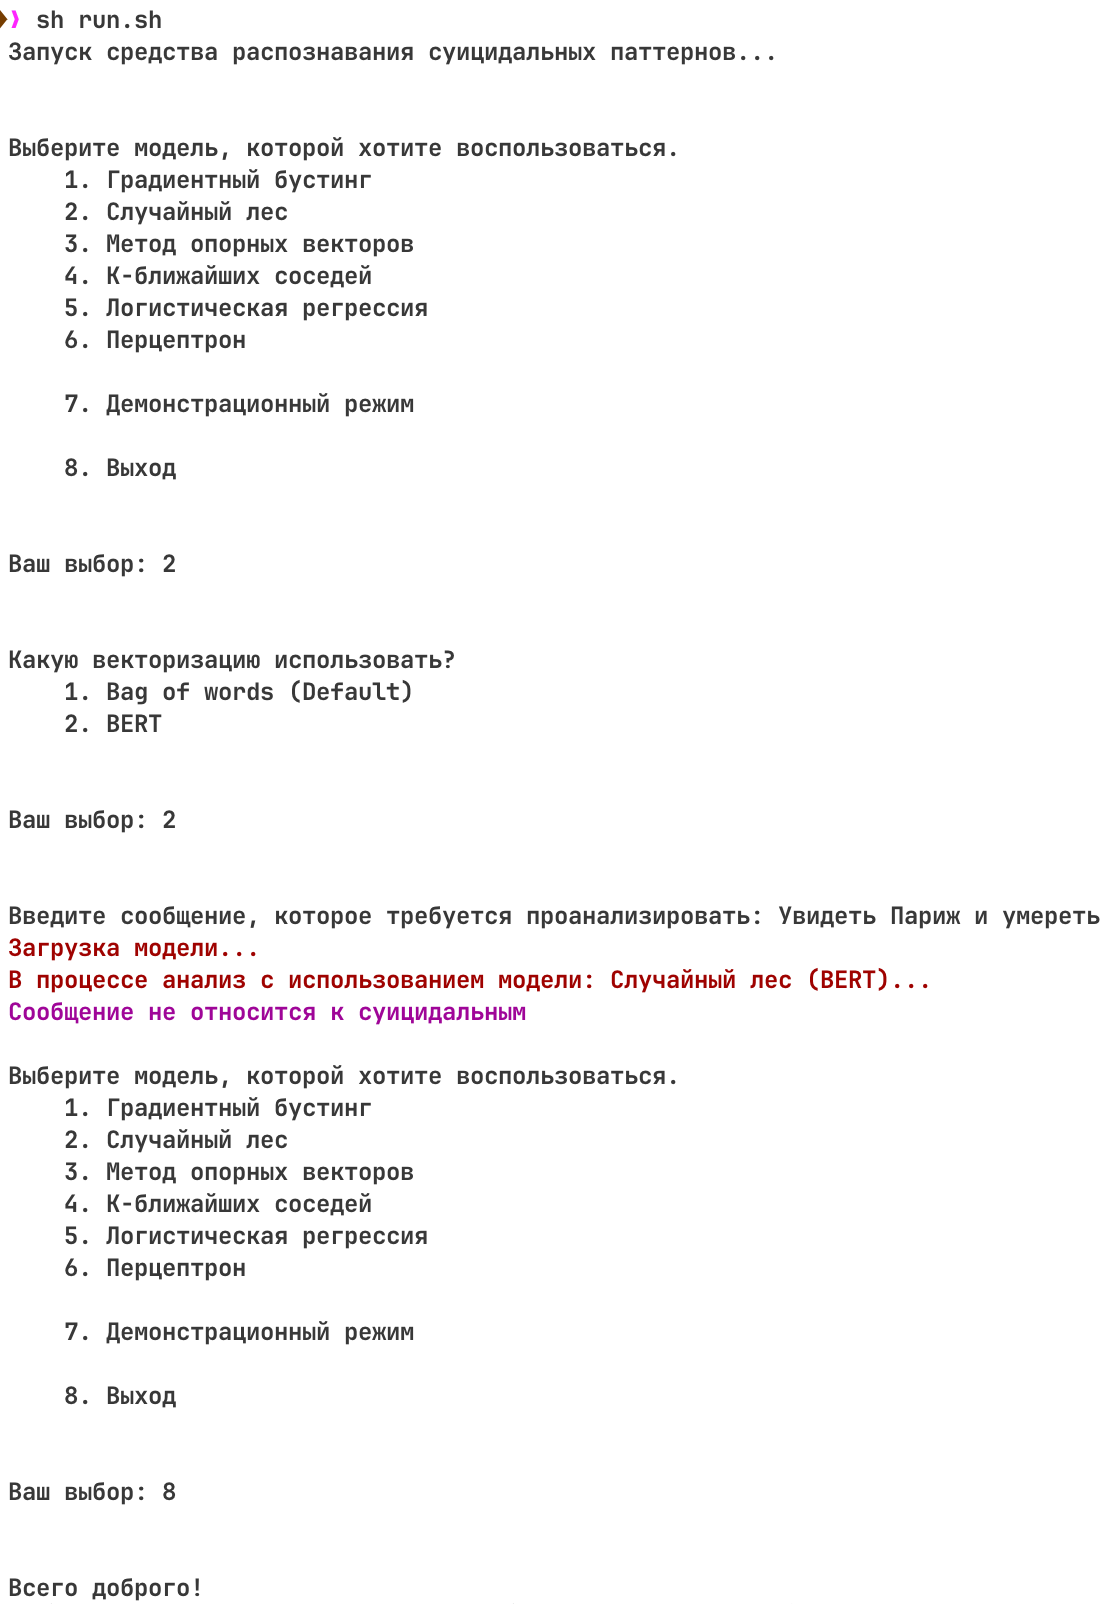
\includegraphics[width=\textwidth]{inc/utility2.png}
	\caption{ Результат анализа суицидального сообщения. }
	\label{img:utility2}
\end{figure}

\begin{figure}[H]
	\centering
	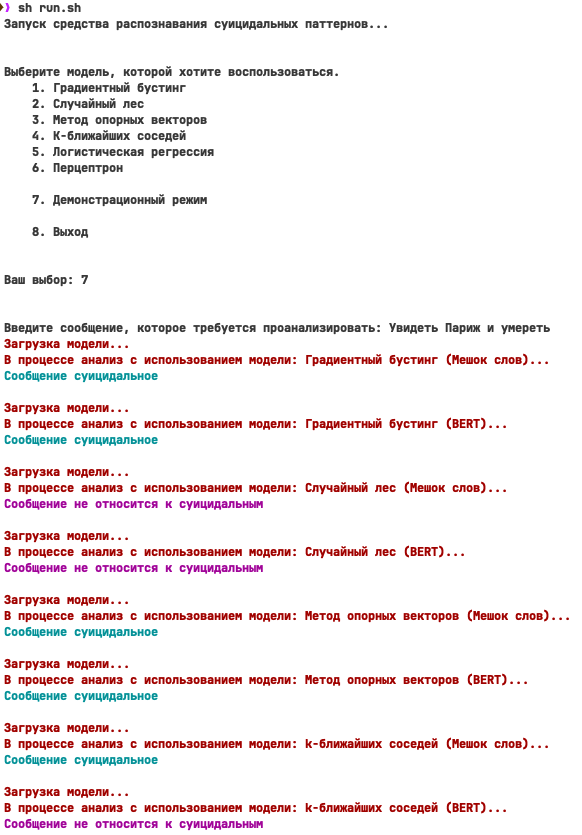
\includegraphics[width=\textwidth]{inc/utility3.png}
	\caption{ Результат демонстрационного запуска. }
	\label{img:utility3}
\end{figure}

\begin{figure}[H]
	\centering
	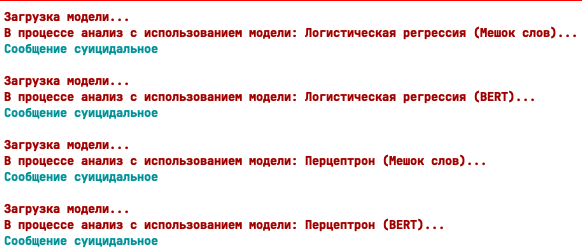
\includegraphics[width=\textwidth]{inc/utility4.png}
	\caption{ Продолжение вывода результатов демонстрационного запуска. }
	\label{img:utility4}
\end{figure}

\subsection{Сведения о модулях}

Программное обеспечение состоит из модулей моделей, векторизаторов, предобработки данных и пользовательского интерфейса.

\textit{Модуль моделей} предназначен для хранения и извлечения обученных моделей для решения поставленных задач.

Библиотеки, используемые в модуле:
\begin{itemize}
	\item Sklearn -- библиотека предоставляет для модуля набор моделей, которые предстоит обучить;
	\item Joblib \cite{joblib} -- библиотека, предоставляющая набор инструментов для облегчения использования python в качестве средства автоматизации; Модуль задействует возможность сохранения объекта Python в виде файла.
\end{itemize}

Модуль состоит из двух пакетов: model и modelprovider. 
Пакет model содержит в себе лишь сохраненные в виде файлов модели.
Пакет modelprovider содержит в себе интерфейс, который должен имплементировать каждый провайдеры, а также сами провайдеры, выполненные по шаблону проектирования ``Одиночка''.


\textit{Модуль векторизаторов} предназначен для хранения и извлечения готовых векторизаторов для решения поставленных задач.

Библиотеки, используемые в модуле:
\begin{itemize}
	\item Sklearn -- библиотека предоставляет для модуля векторизатор, использующий алгоритм ``Мешок слов'';
	\item Transformers \cite{transformers} -- библиотека предоставляет доступ к множеству предобученных моделей;
	\item SciPy \cite{scipy} -- библиотека, предоставляющая реализации множество фундаментальных алгоритмов и структур данных;
	\item Joblib \cite{joblib} -- модуль задействует возможность сохранения объекта Python в виде файла.
\end{itemize}

Модуль состоит из двух пакетов: vectorizer и vectorizerprovider. 
Пакет vectorizer содержит в себе лишь сохраненные в виде файлов модели.
Пакет vectorizerprovider содержит в себе интерфейс, который должен имплементировать каждый провайдеры, а также сами провайдеры, выполненные по шаблону проектирования ``Одиночка''.


\textit{Модуль предобработки данных} предназначен для хранения текущих реализаций средств предобработки данных.

Библиотеки, используемые в модуле:
\begin{itemize}
	\item Pandas -- библиотека задействована для упрощения работы с табличными видами данных;
	\item PyMorphy2 -- библиотека предоставляет морфологический анализатор, позволяющий токенизировать и лемматизировать сообщения, поступающие в систему;
	\item Nltk -- модуль задействует словарь стоп-слов, предоставляемых данной библиотекой.
\end{itemize}

Модуль состоит из трех пакетов: analysis, legacy, prod.
Пакет analysis содержит в себе различные средства анализа датасета и вывода информации о нем.
Пакет legacy задействован для хранения старых и уже незадействованных средств предобработки текстовых сообщений.
Пакет prod содержит в себе актуальные предобработчики данных для различных нужд.

\textit{Модуль пользовательского интерфейса} предназначен для взаимодействия пользователя с другими модулями системы.

Модуль состоит из двух пакетов: console и resources.
Пакет console содержит в себе имплементацию интерфейса пользователя, которая взаимодействует с классом, выполненным по шаблону проектирования ``Фасад''.
Пакет resources предоставляет текстовые ресурсы для интерфейса, он был создан и поддерживается в целях возможности добавления новых поддерживаемых в приложение языков.

\subsection{Описание обрабатываемых данных}

В результате работы средства сбора данных было размечено 1000 суицидальных сообщений. К собранным сообщениям было добавлено еще 1000 несуицидальных сообщений из датасета обнаружения пресуицидальных сигналов~\cite{dataset}. 

На рисунках \ref{img:sentiments1} и \ref{img:sentiments2} представлены круговые диаграммы тональности сообщений, полученные с использованием библиотеки Dostoevsky \cite{dostoevsky}. 

\begin{figure}[H]
	\centering
	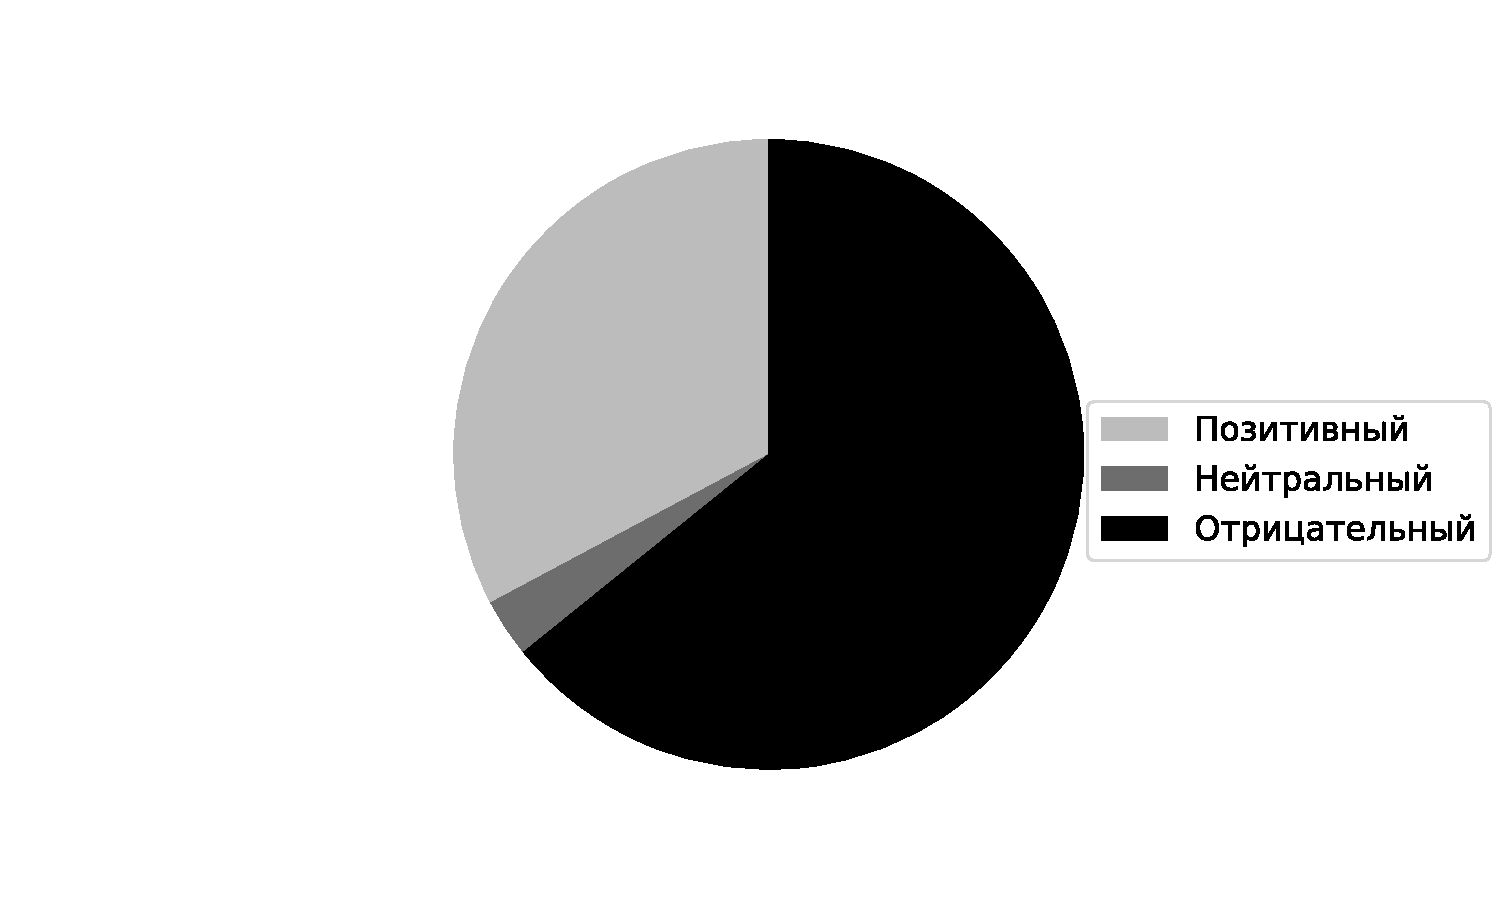
\includegraphics[width=0.9\textwidth]{inc/plots/sentiments_suicidal_monochrome.pdf}
	\caption{ Круговая диаграмма тональности суицидальных сообщений. }
	\label{img:sentiments1}
\end{figure}

\begin{figure}[H]
	\centering
	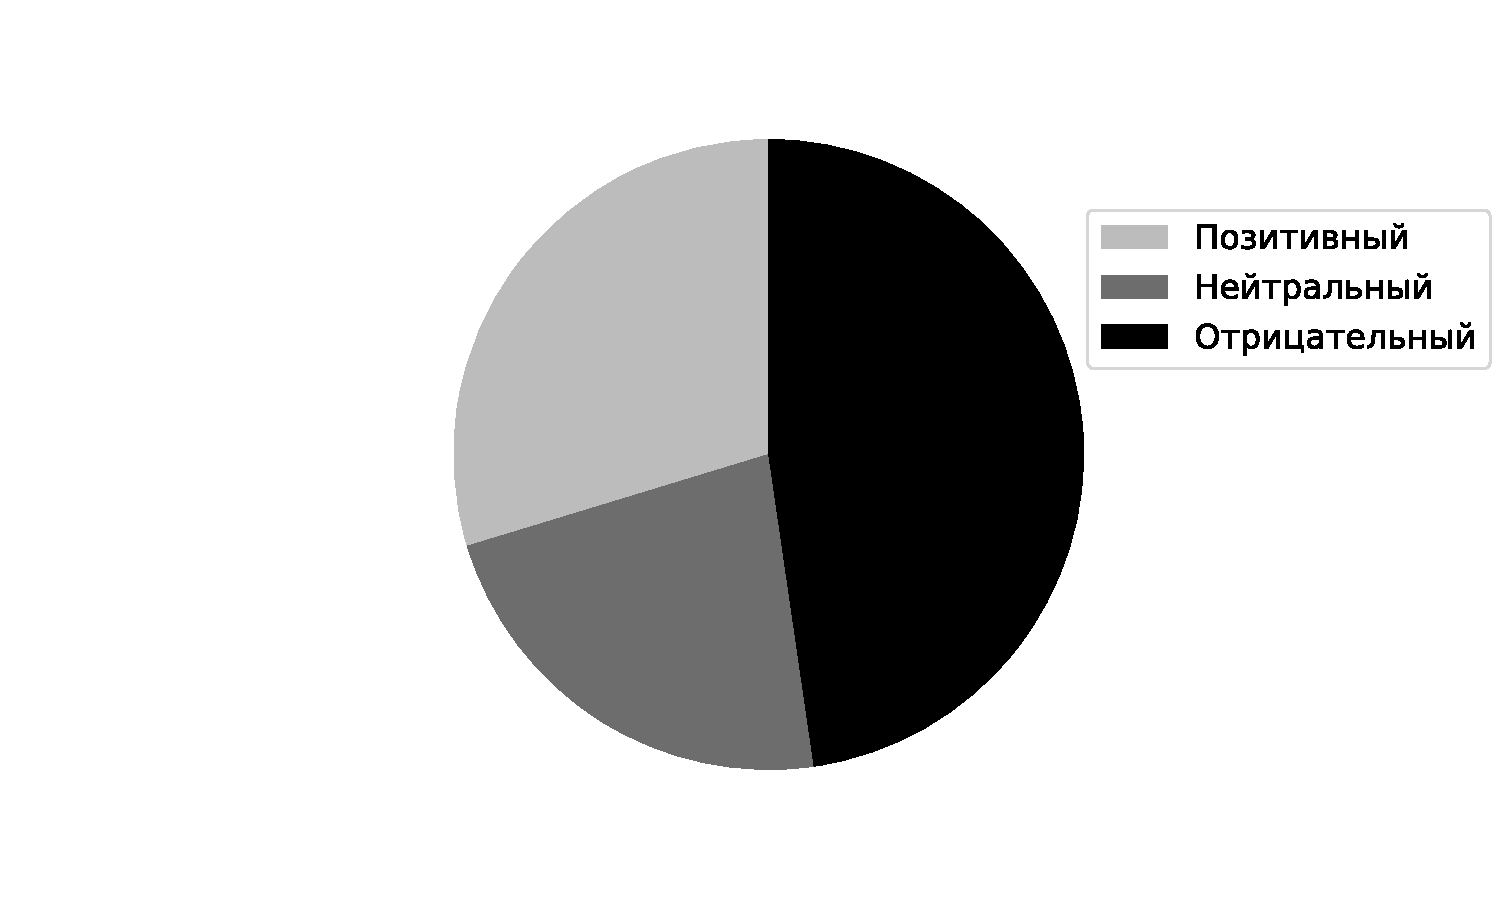
\includegraphics[width=0.9\textwidth]{inc/plots/sentiments_non_suicidal_monochrome.pdf}
	\caption{ Круговая диаграмма тональности несуицидальных сообщений. }
	\label{img:sentiments2}
\end{figure}

Представленные диаграммы показывают, что практически треть суицидальных сообщений автоматизированное средство оценки тональности распознает как сообщения с отрицательной окраской. Однако наличие среди них позитивно настроенных сообщений -- ошибка распознавания модели. Среди несуицидальных сообщений преобладают тексты с отрицательной окраской, однако тут их уже меньше половины, а нейтральных сообщений почти что четверть из всех представленных. 

На рисунке \ref{img:cloud1} представлена визуализация собранных данных класса суицидальных сообщений. Чаще всего в суицидальных сообщениях фигурируют слова ``жизнь'' (585 раз), ``хотеть'' (556 раз), ``человек'' (491 раз) и ``мочь'' (452 раза). Также стоит обратить внимание на присутствие слов ``суицид'', ``страдать'', ``депрессия'', ``смерть'', ``умирать'' и ``ад''.

\begin{figure}[H]
	\centering
	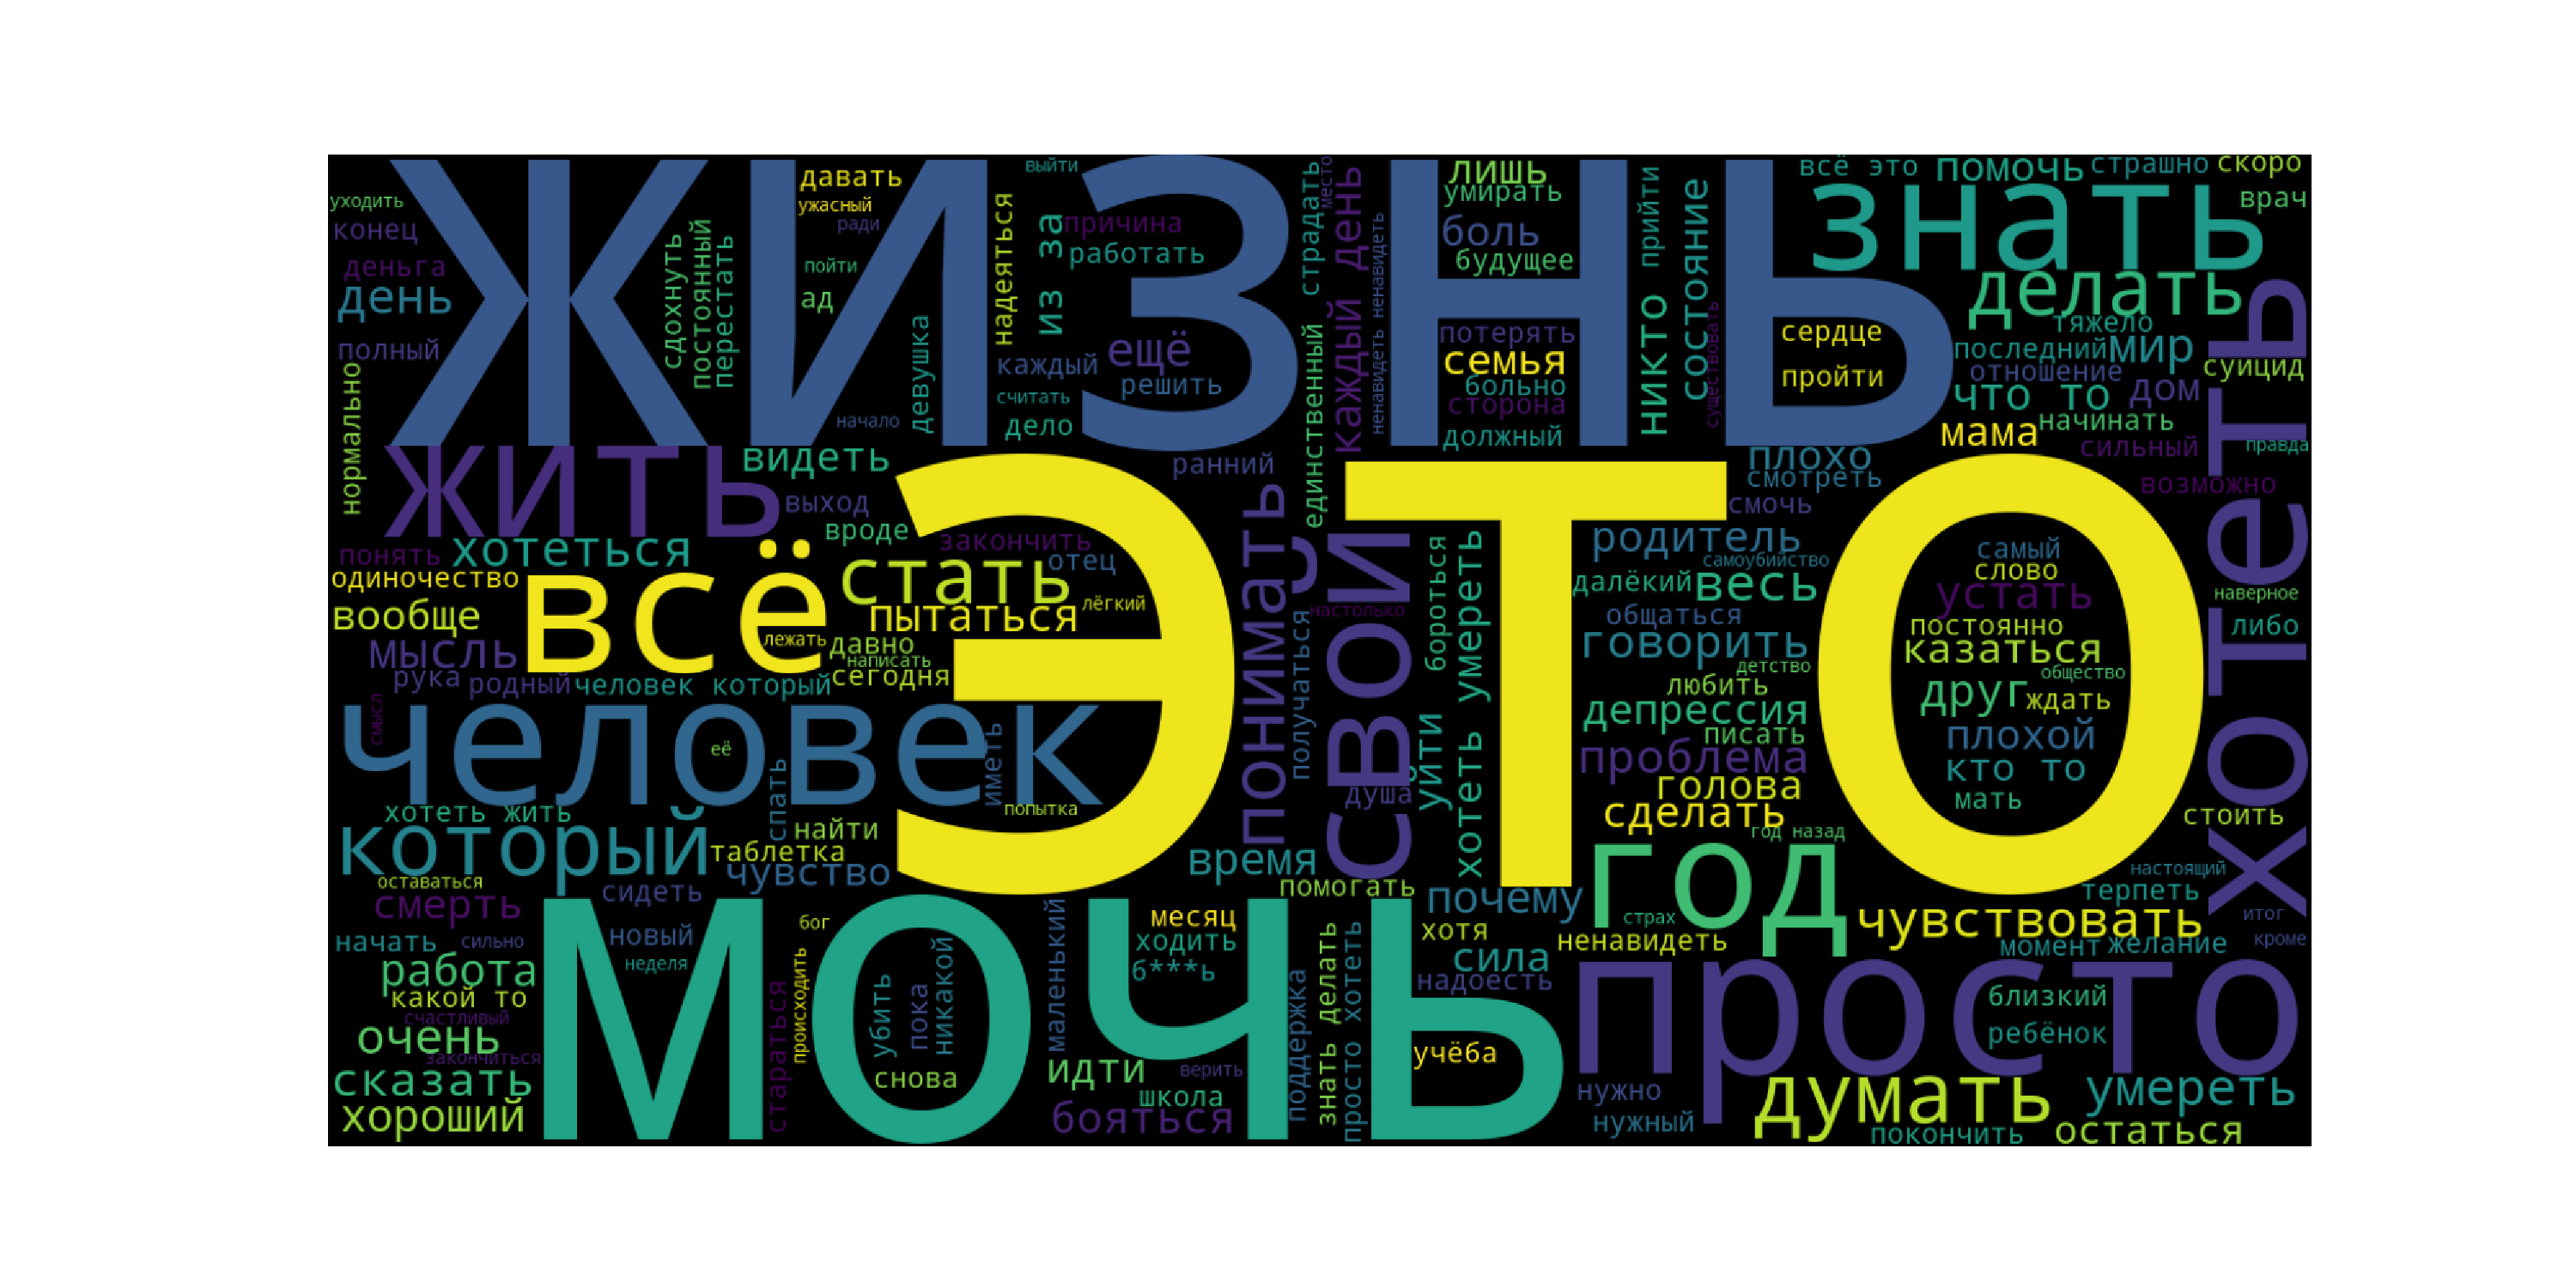
\includegraphics[width=\textwidth]{inc/cloudSuicidal.pdf}
	\caption{ Облако слов класса суицидальных сообщений. }
	\label{img:cloud1}
\end{figure}

На рисунке \ref{img:cloud2} представлена визуализация данных класса несуицидальных сообщений. Чаще всего в несуицидальных сообщениях встречаются слова ``хотеть'' (159 раз) и ``человек'' (67 раз). Кроме того сообщения данной тематики чаще включают в себя различные вариации нецензурной брани.

\begin{figure}[H]
	\centering
	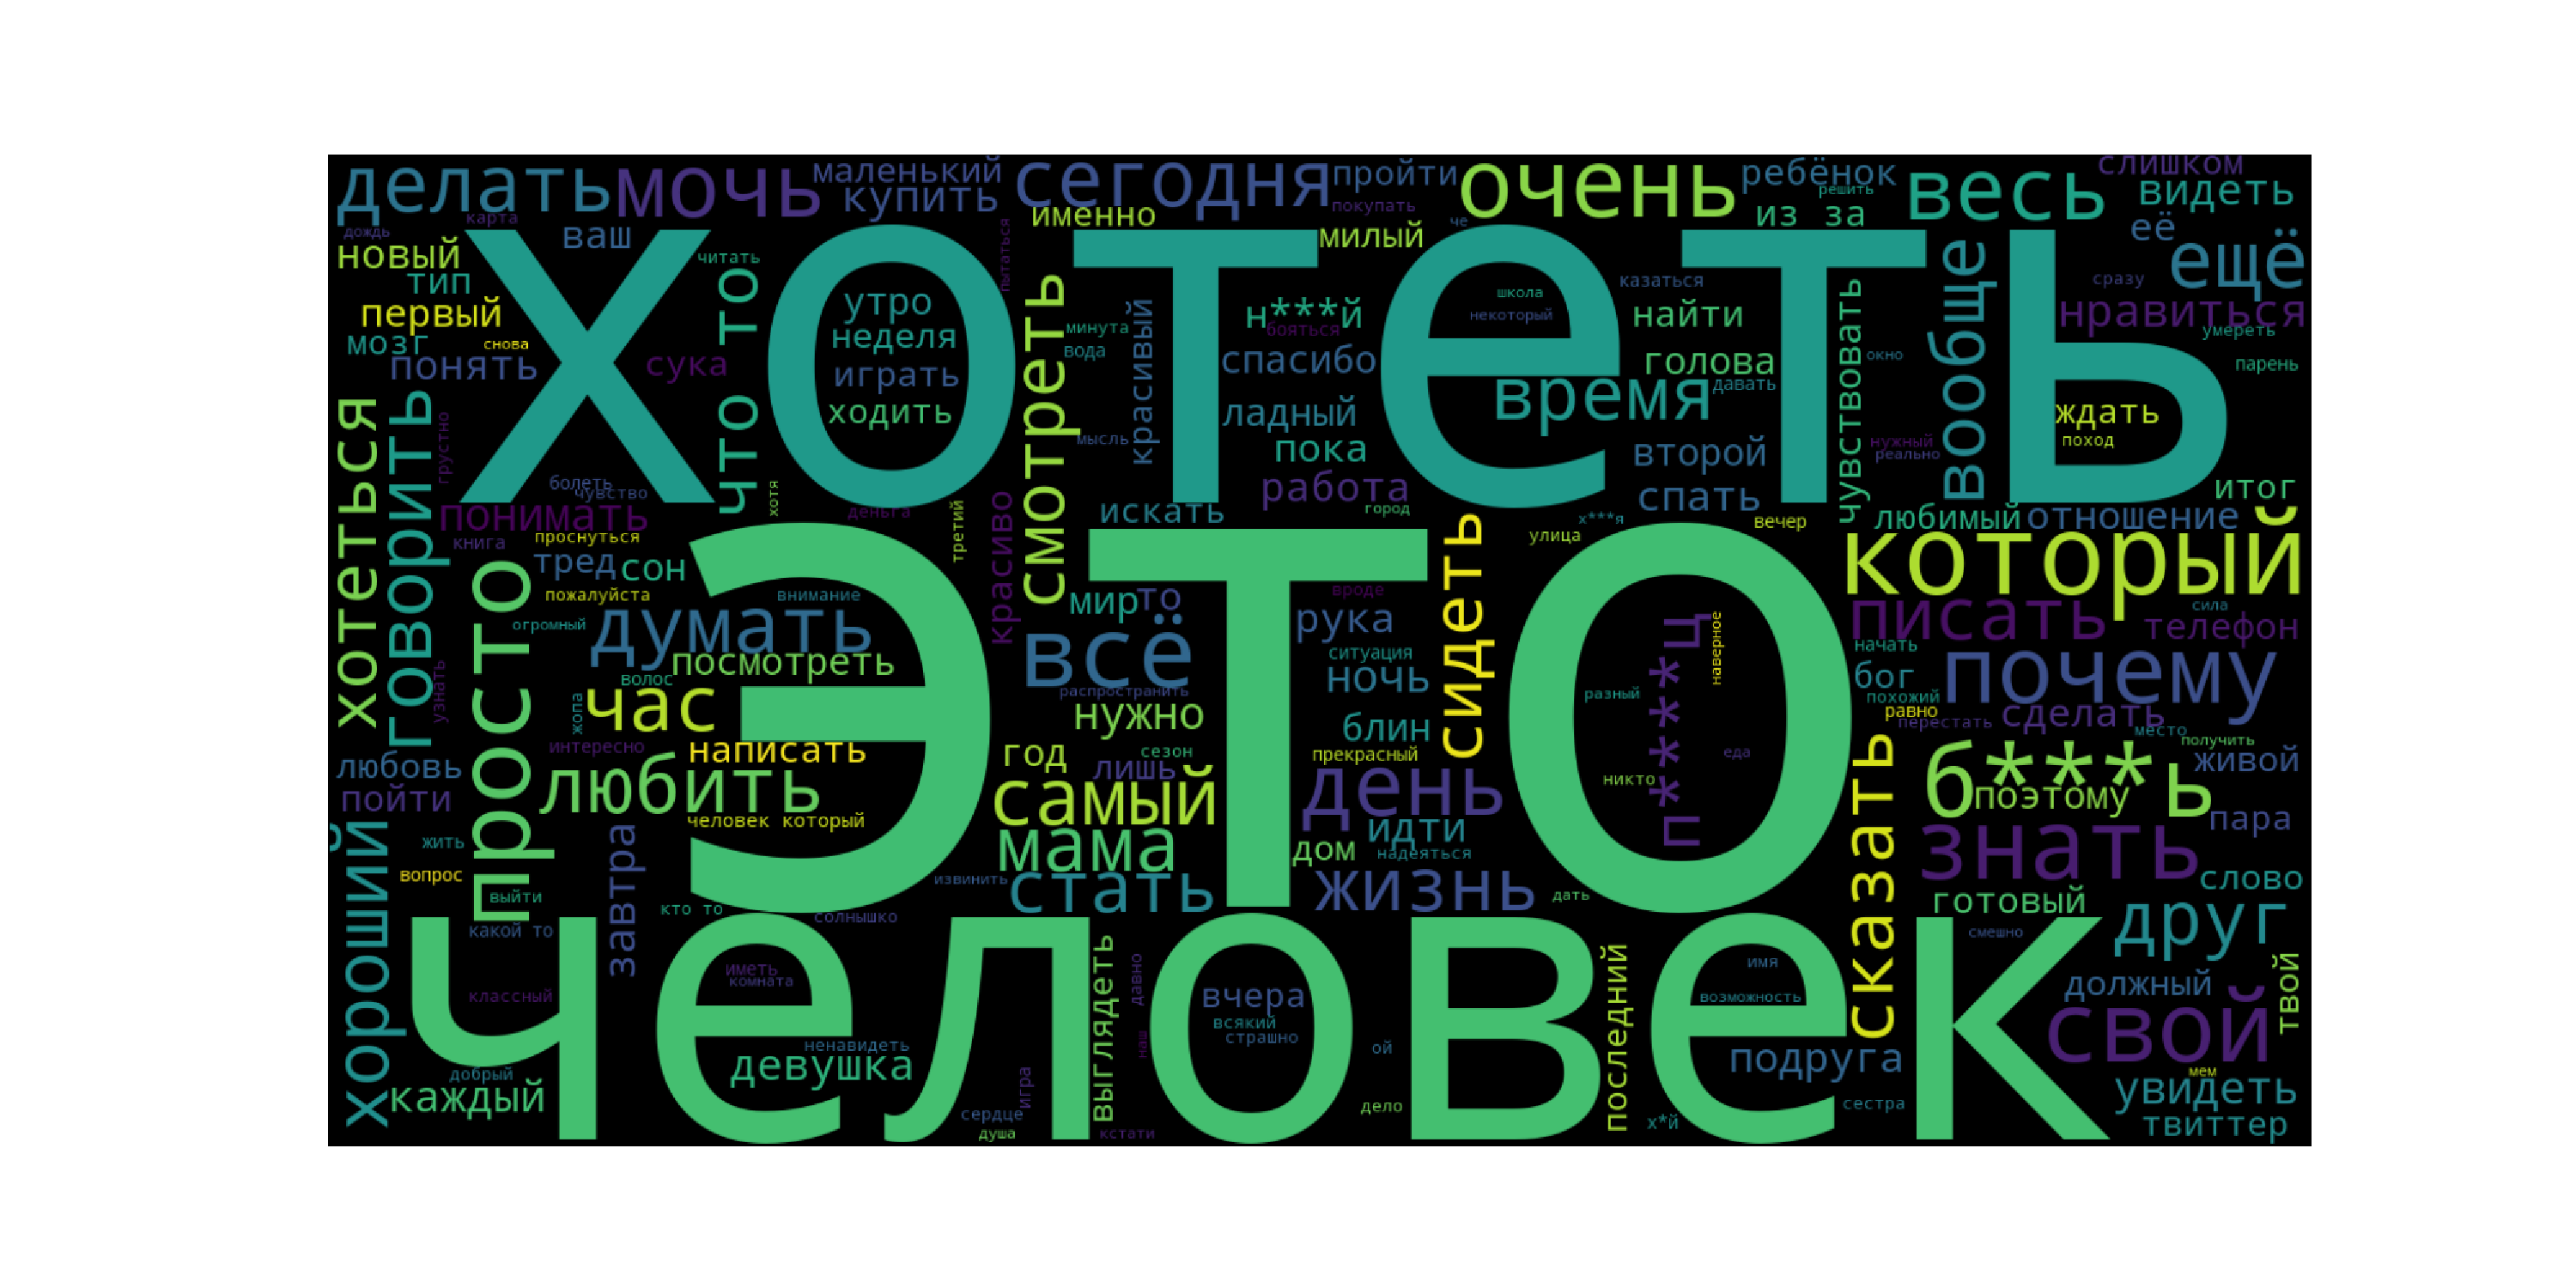
\includegraphics[width=1\textwidth]{inc/cloudNonSuicidal.pdf}
	\caption{ Облако слов класса несуицидальных сообщений. }
	\label{img:cloud2}
\end{figure}

Представленная информация подтверждает факт того, что выбранные классы разделимы и отличны частотой употребления как слов, так и тематик. Кроме того, стоит отметить, что слово ``хотеть'' встречается в суицидальных сообщениях в $\approx 7.83$ раза чаще, чем в несуицидальных, а слово ``человек'' -- в $\approx 7.33$ раза чаще. Таким образом, суицидальные сообщения являются менее ``разнообразными'' и фиксирующимися на определенном словарном множестве.

\subsection*{Вывод}

В качестве инструментов разработки средства сбора данных будут задействованы ЯП Python и библиотека Telebot. 
В качестве языка разработки средства распознавания суицидальных паттернов поведения человека по текстовым сообщениям также будет использоваться ЯП Python. 
Задействованные библиотки: pandas, numpy, matplotlib, scikit-learn, nltk, pymorphy2.

Были представлены интерфейсы средства сбора данных и средства распознавания суицидальных паттернов поведения человека по текстовым сообщениям.
Была приведена информация о модулях системы.

Представленные диаграммы тональности сообщений показали, что практически треть суицидальных сообщений автоматизированное средство оценки тональности распознает как сообщения с отрицательной окраской. 
Среди несуицидальных сообщений преобладают тексты с отрицательной окраской, при этом нейтральных сообщений -- четверть из всех.

Визуализированные облака слов подтвердили гипотезу, что выбранные классы суицидальных и несуицидальных сообщений разделимы и отличны частотой некоторых слов. 
Отмечено, что слово ``хотеть'' встречается в суицидальных сообщениях в $\approx 7.83$ раза чаще, чем в несуицидальных, а слово ``человек'' -- в $\approx 7.33$ раза чаще. 
Таким образом, суицидальные сообщения являются менее ``разнообразными'' и фиксирующимися на определенном словарном множестве.
